\documentclass[utf8]{article}
\usepackage{amsmath,amssymb}
\usepackage{fancyhdr}
\usepackage{graphicx}
\usepackage{fullpage}
\usepackage{setspace}
\usepackage{fancyvrb}
\usepackage{geometry}
\usepackage{lastpage}
\usepackage{lipsum}
\usepackage{float}
\geometry{left=2.5cm, right=2.5cm, top=2cm, bottom=4cm}

\title{\bf\LARGE AI+X Computing Acceleration: From Algorithms Development, Analysis, to Deployment: Final Report}
\author{Yuqi Ren 2022011332 \\ Jinfan Lu 2022010741}
\date{}

\pagestyle{fancy}
\fancyhf{}

\fancyhead[C]{Final Report}
\renewcommand{\headrulewidth}{0.2pt}
\setlength{\headsep}{1cm}

\fancyfoot[R]{Page \thepage\ of \pageref{LastPage}}
\renewcommand{\footrulewidth}{0.2pt}
\setlength{\footskip}{1.5cm}

\begin{document}
\maketitle
\thispagestyle{empty}

\section{Introduction}

In this project, we have implemented two advanced network topologies, SlimFly and DragonFly, alongside their corresponding routing algorithms and a deadlock-avoidance technique that utilizes virtual channels. SlimFly and DragonFly are among the most efficient topologies, with diameters of two and three, respectively.

\section{Architecture}
\subsection{Topology}
\begin{itemize}
    \item \textbf{SlimFly}: The SlimFly topology is characterized by a highly symmetric internal structure, consisting of two subgraphs, each composed of identical subgroups of routers. As depicted in Figure 1, the first subgraph consists of routers \((0,x,y)\), while the second is formed by routers \((1,m,c)\). These two subgraphs comprise \(q\) subgraphs that do not directly connect with each other, with each subgraph containing \(q\) routers. Router $(0, x, y)$ and router $(1, m, c)$ are connected if and only if $y = mx + c$.

    \begin{figure}[h]
        \centering
        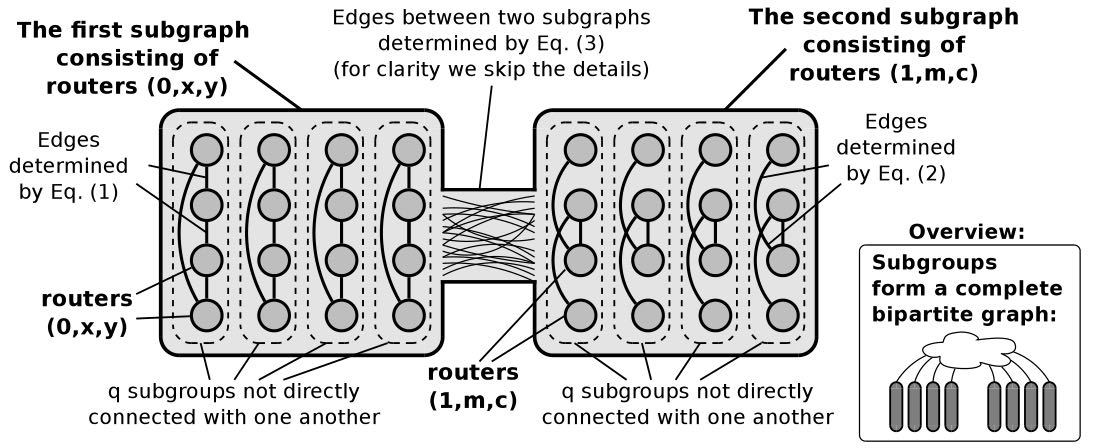
\includegraphics[width=0.7\linewidth]{SlimFly.png}
        \caption{SlimFly topology}
    \end{figure}

    Based on this topology, we can derive several key metrics: Diameter = \(2\), Degree = \(O(q)\), Average Distance \(\approx 2\), and Cost = \(O(q^3)\).

    \item \textbf{DragonFly}: The DragonFly topology is a hierarchical network organized into three levels: system, group, and router. At the group level, \(n\) routers within the same group are fully interconnected. At the system level, there are \(m\) groups, and each pair of groups is connected by a single link. Specifically, the \(i\)-th group and the \(j\)-th group are connected via global channels between the \((i \mathrm{~mod~} n)\)-th router in group \(j\) and the \((j-1 \mathrm{~mod~} n)\)-th router in group \(i\). From this topology, we can compute the following metrics: Diameter = \(3\), Degree \(\le n-1+\lceil m/n\rceil\), Average Distance \(\approx 3\), and Cost = \(O(n^2m)\). An example of a special DragonFly topology (\(m=2n+1\)) is shown in Figure 2.

    \begin{figure}[h]
        \centering
        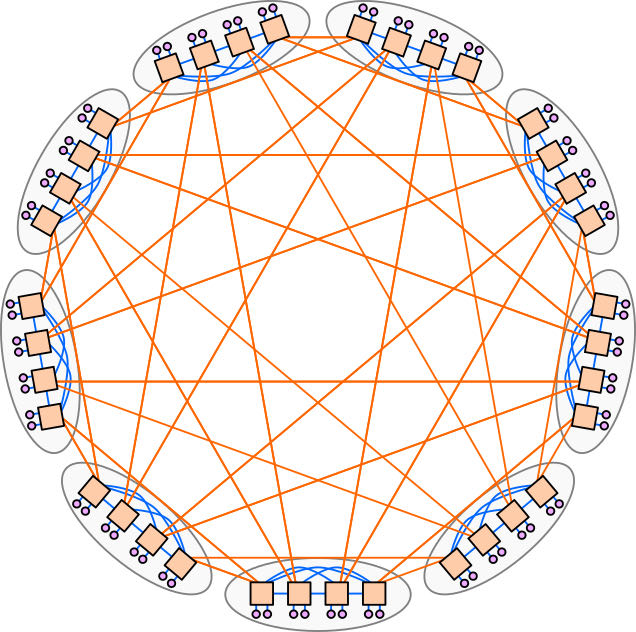
\includegraphics[width=0.4\linewidth]{DragonFly.png}
        \caption{DragonFly topology}
    \end{figure}
\end{itemize}

\subsection{Routing}
We have implemented two fundamental routing methods for the DragonFly and SlimFly topologies:
\begin{itemize}
    \item \textbf{Minimal Static Routing}: In minimal routing, a packet is forwarded along the shortest path from the source router \(R_s\) to the destination router \(R_d\).
    \item \textbf{Valiant Random Routing}: In Valiant routing, the protocol first randomly selects an intermediate router \(R_r\). The packet is then routed from the source router \(R_s\) to the intermediate router \(R_r\), and finally from \(R_r\) to the destination router \(R_d\). The resulting paths may consist of 2, 3, or 4 hops.
\end{itemize}

\subsection{Deadlock Freedom}
To ensure deadlock avoidance in SlimFly, we implement a technique that utilizes virtual channels. When sending a packet from router \(R_a\) to \(R_b\), if they are directly connected, virtual channel \(VC_0\) is used. Otherwise, as the maximum distance in SlimFly is two hops, virtual channel \(VC_0\) is used for the first hop and \(VC_1\) for the second hop. This approach effectively breaks cycles into different sets of buffers, thus preventing deadlocks.

\section{Implementation}

\subsection{Topology}
\begin{itemize}
    \item \textbf{SlimFly Topology}: The implementation of SlimFly involves two main steps: adding intra-group links and inter-group links. First, we divide routers into groups based on their indices. Then, we connect router \((0,x,y)\) with router \((0,x,y^\prime)\) if \(y-y^\prime \in X\), and connect router \((1,m,c)\) with router \((1,m^\prime,c^\prime)\) if \(c-c^\prime \in Y\), where \(X=\{1,\xi^2, \dots, \xi^{q-3}\}\), \(Y=\{\xi, \xi^3, \dots, \xi^{q-2}\}\), and \(\xi\) is an element of the Galois Field \(\mathbb{F}_q\) that generates \(\mathbb{F}_q\). Finally, we add inter-group links by connecting router \((0,x,y)\) with router \((1,m,c)\) if and only if \(y=mx+c\).

    In our implementation, considering a configuration with 64 CPUs, we set \(q=5\), resulting in 50 routers. Therefore, we have \(X = \{1, 4\}\) and \(X'=\{2, 3\}\).

    \item \textbf{DragonFly Topology}: The implementation of DragonFly follows a similar approach as SlimFly. We first add intra-group links and then inter-group links. Denoting the \(i\)-th router in group \(j\) as \((i,j)\), we add inter-group links as follows: connect router \((j-1 \mathrm{~mod~} n, i)\) with router \((i \mathrm{~mod~} n, j)\).
\end{itemize}

\subsection{Routing}
\begin{itemize}
    \item \textbf{Minimal Static Routing}: To find the shortest path, we assign a weight of 1 to all links in the network. Since the function \texttt{lookupRoutingTable} in \texttt{RoutingUnit.cc} will select the path of smallest weight, we can directly call it and then get the shortest path.
    \item \textbf{Valiant Random Routing}: To select the intermediate router, we define a random selection mechanism that balances traffic. Specifically, we add a member variable \texttt{mid\_router} to class \texttt{RouteInfo} in \texttt{src/mem/ruby/network/garnet/CommonTypes.hh} and decide the path in \texttt{RoutingUnit.cc}.
\end{itemize}

\subsection{Deadlock Freedom}

In our implementation, we set the number of virtual channels to 2. When sending a packet, we check whether the destination router is directly connected. If it is, we use \(VC_0\); otherwise, we use \(VC_0\) for the first hop and \(VC_1\) for the second hop.

These modifications primarily involved changes in \texttt{src/mem/ruby/network/garnet/OutputUnit.cc}, particularly in the logic of the \texttt{has\_free\_vc} and \texttt{select\_free\_vc} functions, which are responsible for managing the availability and selection of virtual channels.

\section{Experiments and Analysis}

\subsection{Topology}

\begin{figure}[H]
    \centering
    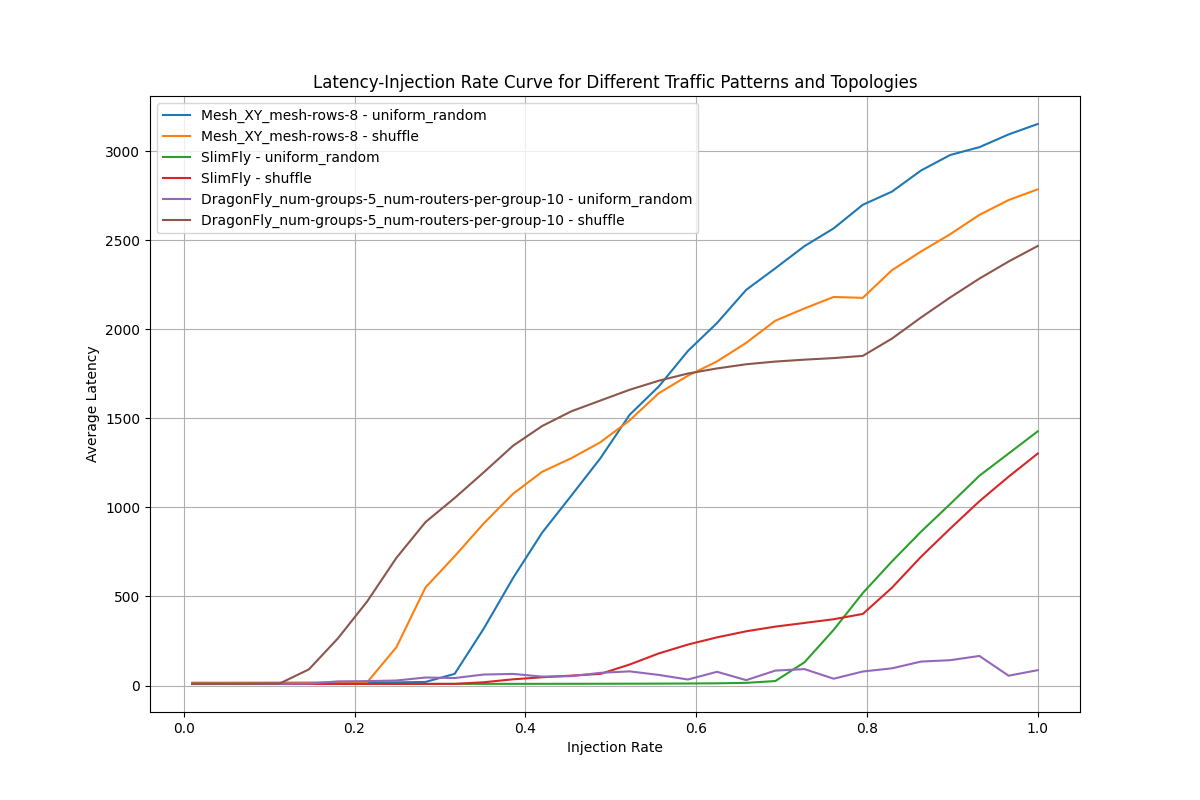
\includegraphics[width=0.85\linewidth]{topology_1.png}
    \caption{Experiemnts of topology}
\end{figure}

\begin{figure}[H]
    \centering
    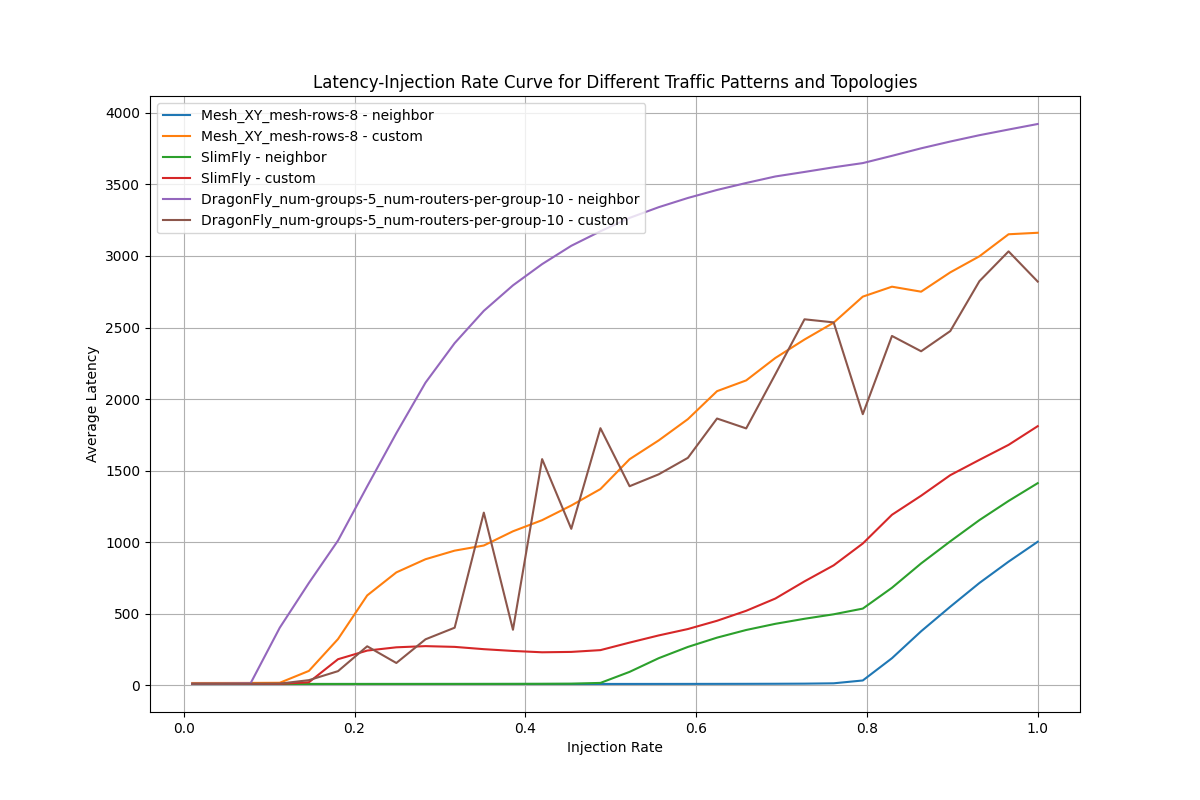
\includegraphics[width=0.85\linewidth]{topology_2.png}
    \caption{Experiemnts of topology}
\end{figure}

As illustrated in Figures 3 and 4, we conducted experiments comparing the average latency of different topologies—Mesh\_XY, SlimFly, and DragonFly—under the default minimal routing algorithm. SlimFly demonstrated superior performance across all synthetic traffic patterns, attributed to its small diameter of 2, which minimizes the number of hops required. DragonFly showed its advantage primarily under uniform random traffic, but it suffered from congestion under other synthetic traffic patterns. Mesh\_XY performed well only in neighbor traffic, as its structure allows neighboring nodes to reach each other in just one hop. These results highlight the robustness of the SlimFly topology, which maintained good performance across various traffic scenarios.

\subsection{Routing}

\begin{figure}[H]
    \centering
    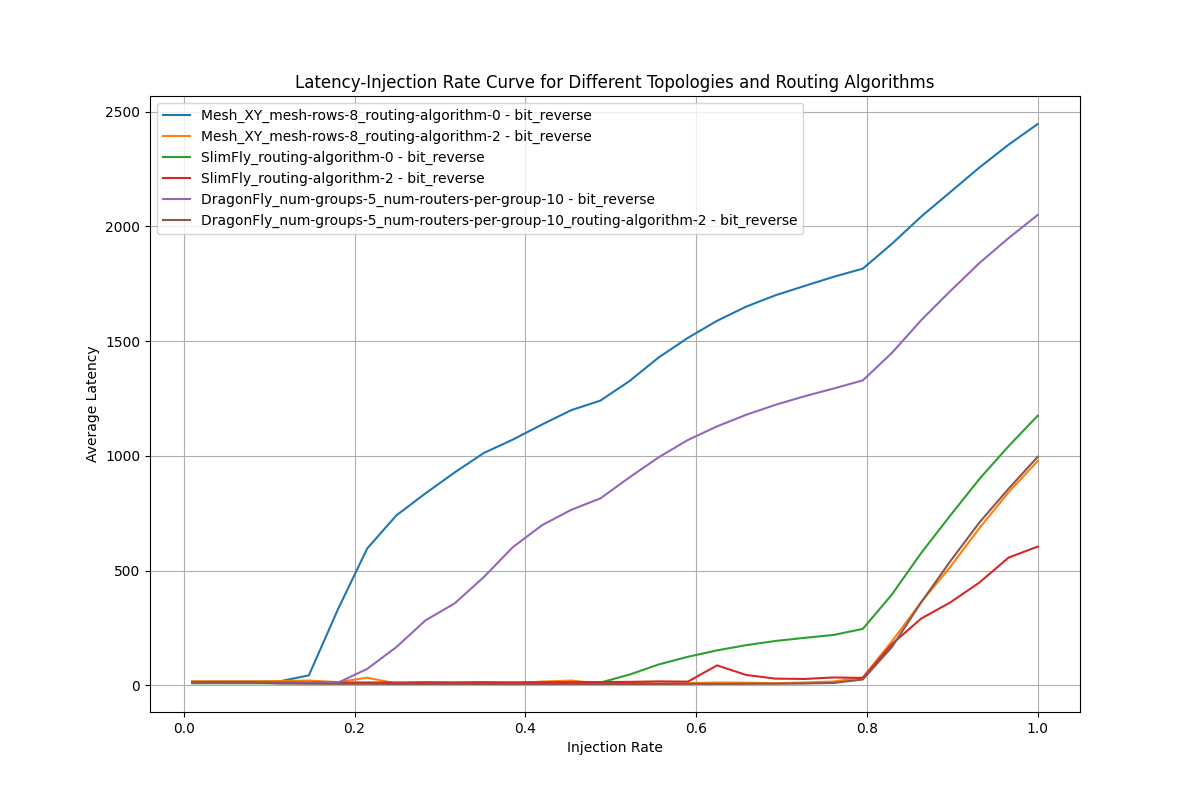
\includegraphics[width=0.85\linewidth]{routing.png}
    \caption{Experiemnts of routing}
\end{figure}

In the routing section, we implemented Valiant Random Routing. In the chart, \texttt{routing-algorithm=0} represents Minimal Static Routing, and \texttt{routing-algorithm=2} corresponds to Valiant Random Routing. It is evident from the results that our newly implemented algorithm significantly reduced congestion. While it introduces a slight increase in low-injection latency, it effectively alleviates the risk of deadlocks and congestion, offering a more stable and efficient routing solution.

\subsection{Deadlock Freedom}

To evaluate the effectiveness of the deadlock-avoidance technique, we conducted simulations with and without the deadlock prevention algorithm. The built-in synthetic traffic patterns in Garnet are not suitable for detecting deadlocks in SlimFly, so we implemented a custom synthetic traffic pattern. In this pattern, most packets follow a specific path \((R_x, R_y)\), which is clearly illustrated below.

\begin{figure}[H]
    \centering
    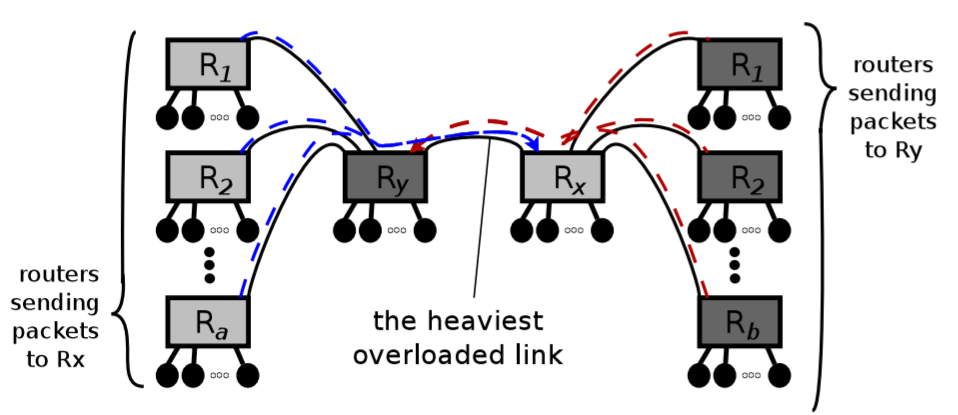
\includegraphics[width=0.6\linewidth]{WorstCase.png}
    \caption{Illustration of the worst-case scenario for SlimFly}
\end{figure}

\begin{figure}[H]
    \centering
    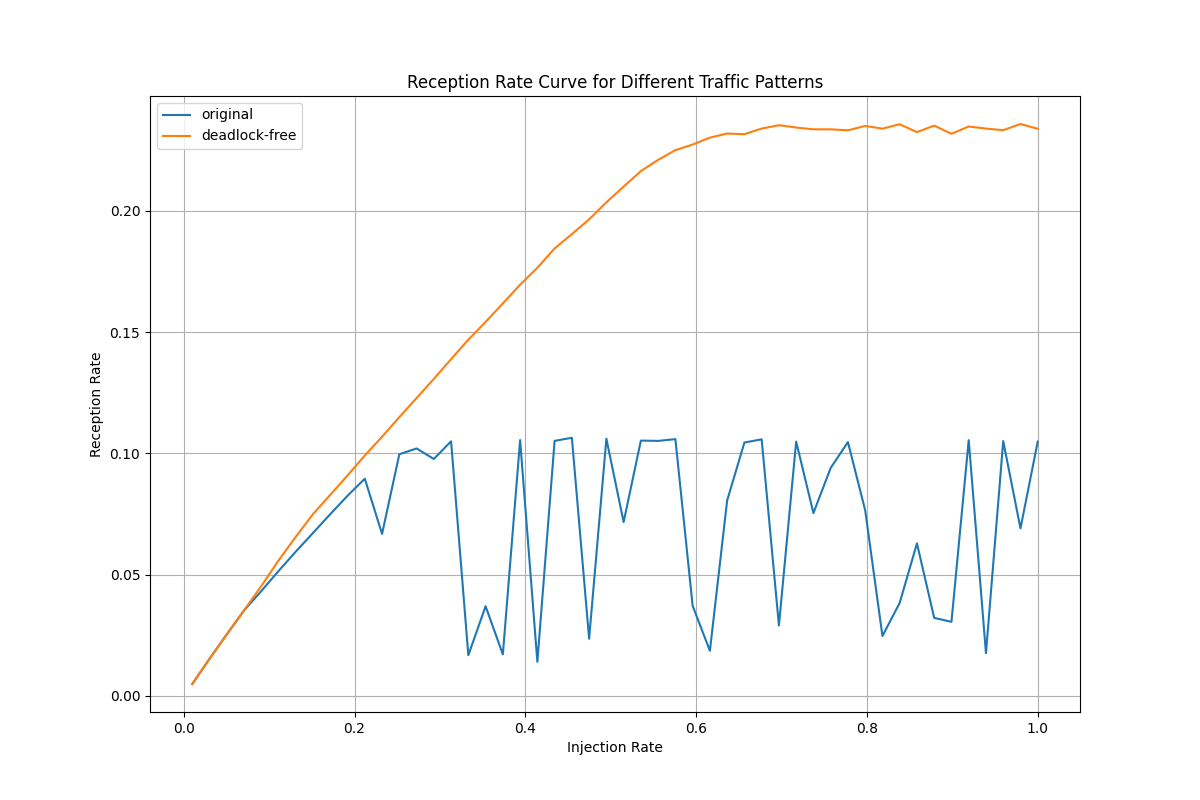
\includegraphics[width=0.85\linewidth]{deadlock.png}
    \caption{Experiemnts of deadlock free algorithm}
\end{figure}

We use reception rate to indicate the occurrence of deadlocks in the minimal static routing algorithm. The original algorithm shows some points with extremely low reception rates, indicating deadlocks. Due to the inherent randomness in our synthetic traffic pattern, some areas may still exhibit higher reception rates.

\section{Labor distribution}
Yuqi Ren (50\%):
\begin{itemize}
    \item Paper reading (SlimFly, DragonFly)
    \item DragonFly topology
    \item Minimal routing, Valiant random routing
    \item Experiments (50\%)
    \item Report (Topology, Routing)
    \item PPT, Pre
\end{itemize}
Jinfan Lu (50\%):
\begin{itemize}
    \item Paper reading (SlimFly, deadlock)
    \item SlimFly topology
    \item Valiant random routing
    \item Experiments (50\%)
    \item Report (deadlock)
    \item PPT, Pre
\end{itemize}
In summary, we complete the entire project with equal contributions.

\section{Reference}
\begin{itemize}
    \item Besta, Maciej, and Torsten Hoefler. "Slim fly: A cost effective low-diameter network topology." SC'14: proceedings of the international conference for high performance computing, networking, storage and analysis. IEEE, 2014.
    \item Kim, John, et al. "Technology-driven, highly-scalable dragonfly topology." ACM SIGARCH Computer Architecture News 36.3 (2008): 77-88.
    \item Besta, Maciej, et al. "Slim noc: A low-diameter on-chip network topology for high energy efficiency and scalability." ACM SIGPLAN Notices 53.2 (2018): 43-55.
\end{itemize}

\section*{Appendix (How to Reproduce Experimental Results)}
\begin{Verbatim}[frame=single]
    # 1: Install Dependencies
    sudo apt install build-essential git m4 scons zlib1g zlib1g-dev \
    libprotobuf-dev protobuf-compiler libprotoc-dev libgoogle-perftools-dev \
    python3-dev libboost-all-dev pkg-config

    # 2: Build
    git clone https://github.com/gem5/gem5
    cd gem5
    git checkout v23.0.0.1
    # replace /path/to/lab4.patch with the actual path of lab4.patch
    git apply /path/to/lab4.patch
    pip install -r requirements.txt
    scons build/NULL/gem5.opt PROTOCOL=Garnet_standalone -j $(nproc)

    # 3: Run
    python ./experiemnts/topology_1.py      # Figure 3
    python ./experiemnts/topology_2.py      # Figure 4
    python ./experiemnts/routing.py         # Figure 5
    python ./experiemnts/deadlock.py        # Figure 7

\end{Verbatim}

\end{document}
